\documentclass[a4paper, 11pt]{article}
\usepackage{comment} 
\usepackage{fullpage}
\usepackage{amsmath} 
\usepackage{amssymb} 
\usepackage{mathtools}
\usepackage{fontspec}
\usepackage{siunitx}
\defaultfontfeatures{Ligatures=TeX}
\usepackage{xfrac}
\usepackage{icomma}
\usepackage[section,below]{placeins}
\usepackage[labelfont=bf,font=small,width=0.9\textwidth]{caption}
\usepackage{subcaption}
\usepackage{graphicx}
\usepackage{grffile}
\usepackage{float}
\floatplacement{figure}{htbp}
\floatplacement{table}{htbp}
\usepackage{booktabs}
\usepackage{hyperref}
\begin{document}
\noindent
\centerline{\small{\textsc{Michigan State University}}} \\
\large{\textbf{CMSE/CSE 822 – Parallel Computing \hfill Fall 2019 \\
Homework 4}} \\
Alexander Harnisch \\
\noindent\makebox[\linewidth]{\rule{\textwidth}{0.4pt}}

\section*{1) OpenMP Parallel Sparse Matrix Vector Multiplication}
You might notice that I do not set the number of threads in the code. I set the
number of threads by requesting the according number of cores in the job
script, which I dynamically generate from a template. I wrote the parallel code
in a general way, letting the OpenMP runtime choose the amount of threads it
spawns. Usually for the code I wrote that should be equal to the number of
available cores.
 
\subsection*{a) Parallel Matrix Conversion Code}
I found it to be quite hard to achieve a significant speedup here. Most loops
are not worth paralyzing. The most significant speedup arises from paralyzing
the loop which calculates the number of non zero elements per block for the CSB
format. Here I simply paralyze the outer loop which iterates over all columns. 

The loop after that which allocates the memory for all blocks is also worth
paralyzing. To make things a little more efficient it makes sense to collapse
the two most outer loops. That leads to each individual block being a chunk of
work that can be executed by a single thread. 

I also paralyzed the following loop but it doesn't seem to make a significant
difference.

\subsection*{b) Parallel Sparse Matrix Vector Multiplication using the CSC Format}
Simply paralyzing the outer loop iterating over all columns leads to the best
results of all different ways I have tested. It seems like for large matrices
there are enough columns to efficiently distribute the work and it keeps the
overhead very low since there are no data conflicts when writing to the $b$
output vector in this way. However, since the time measurements are biased due
to cache utilization of the parallel version after executing the sequential
version on the same input, it is hard to provide a solid assessment here.

\subsection*{c) Parallel Sparse Matrix Vector Multiplication using the CSB Format}
This one was actually the most complicated to efficiently paralyze. The most
efficient way I found is based on paralyzing all blocks by collapsing the two
outer loops. However, this creates writing conflicts into the output vector
between all threads. The most efficient way to resolve this is to provide each
thread with it's own copy of an empty output vector and summing them up
afterwards, which is exactly what I did.

\subsection*{d) Results for Three Large Matrices}
The requested plots are provided by Figure~\ref{fig:it-2004} for the
\textit{it-2004} matrix, Figure~\ref{fig:sk-2005} for \textit{sk-2005} and
Figure~\ref{fig:twitter7} for the \textit{twitter7} matrix. All plots contain a
horizontal black line as a reference for no speedup ($y$-value of 1).
\begin{figure}
  \centering
  \makebox[\textwidth][c]{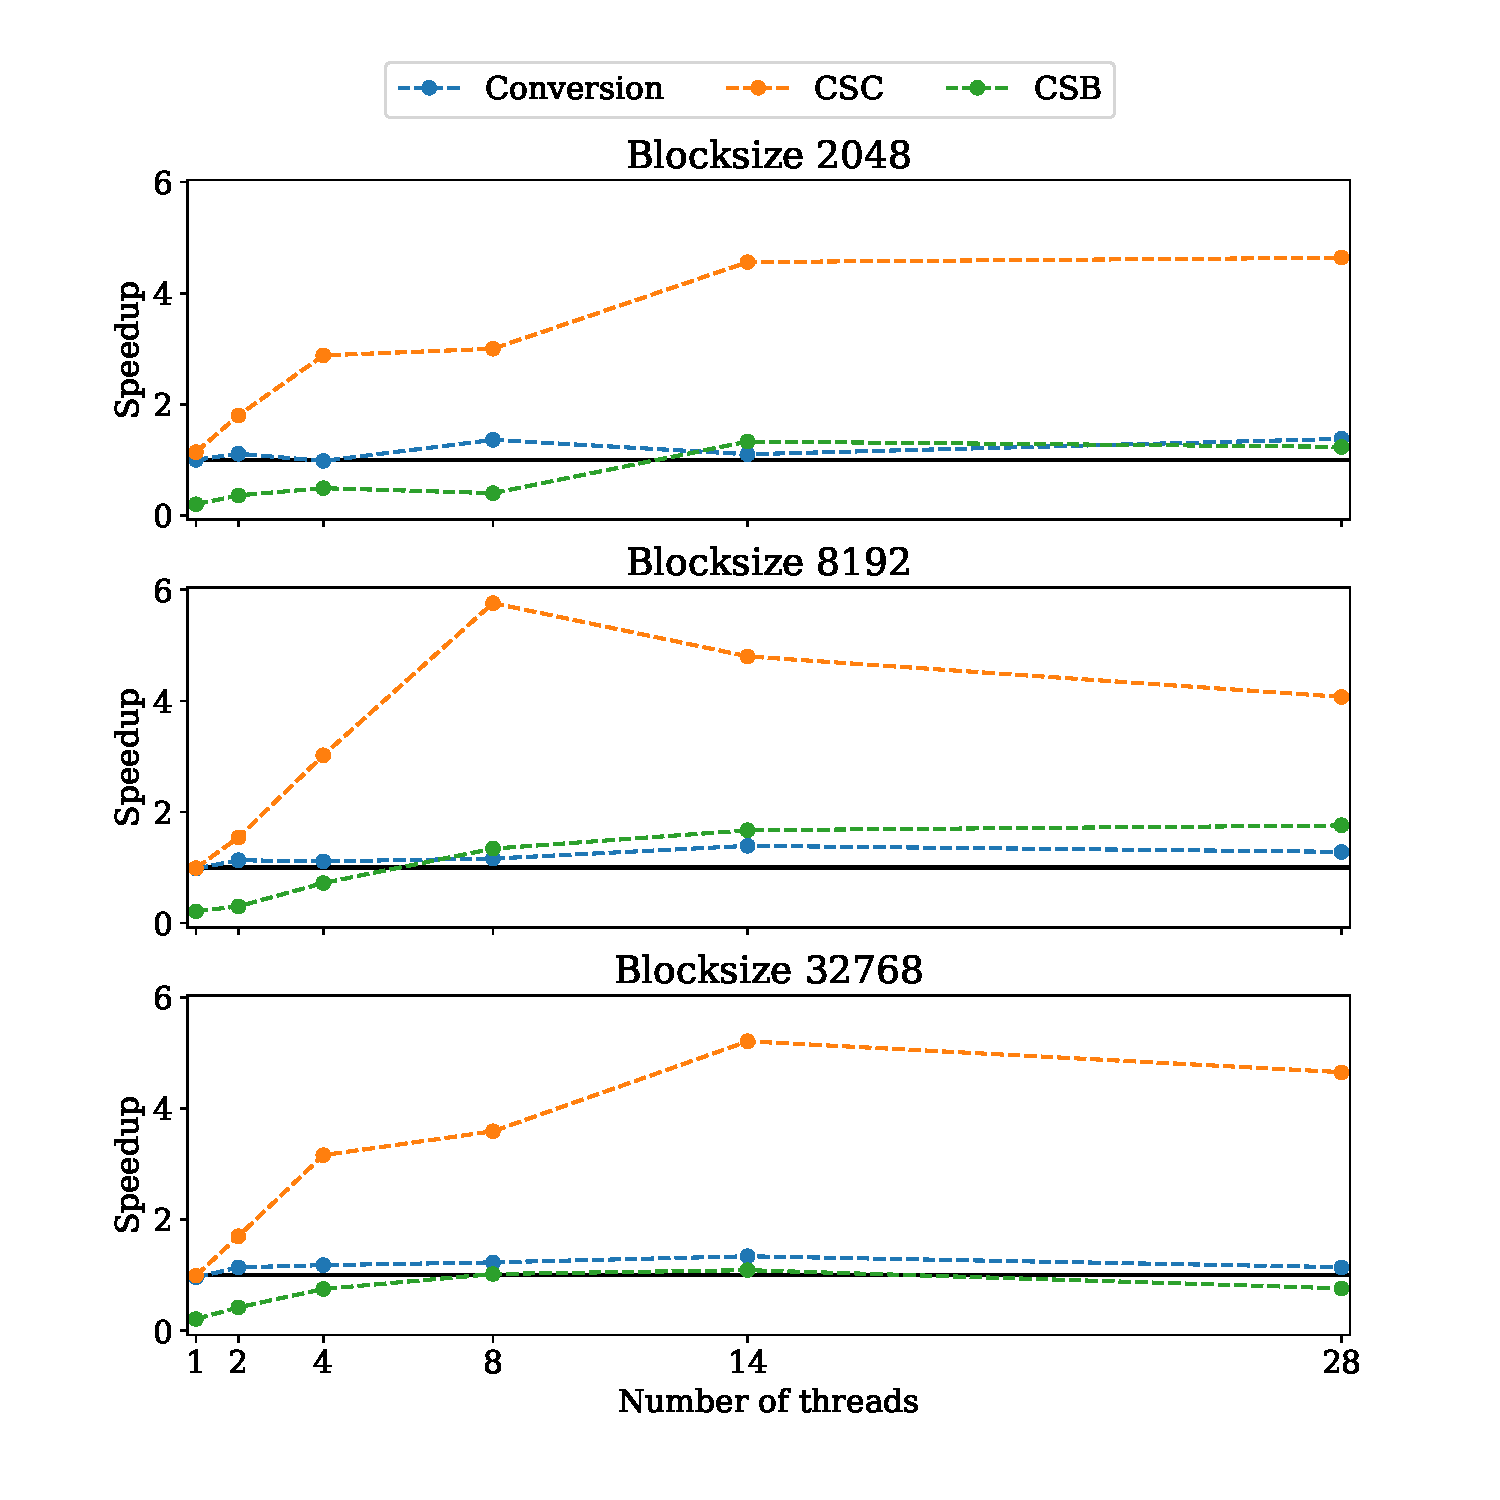
\includegraphics[width=1.4\textwidth]{../plot/it-2004.pdf}}%
  \caption{Results for the \textit{it-2004} matrix.}
  \label{fig:it-2004}
\end{figure}
\begin{figure}
  \centering
  \makebox[\textwidth][c]{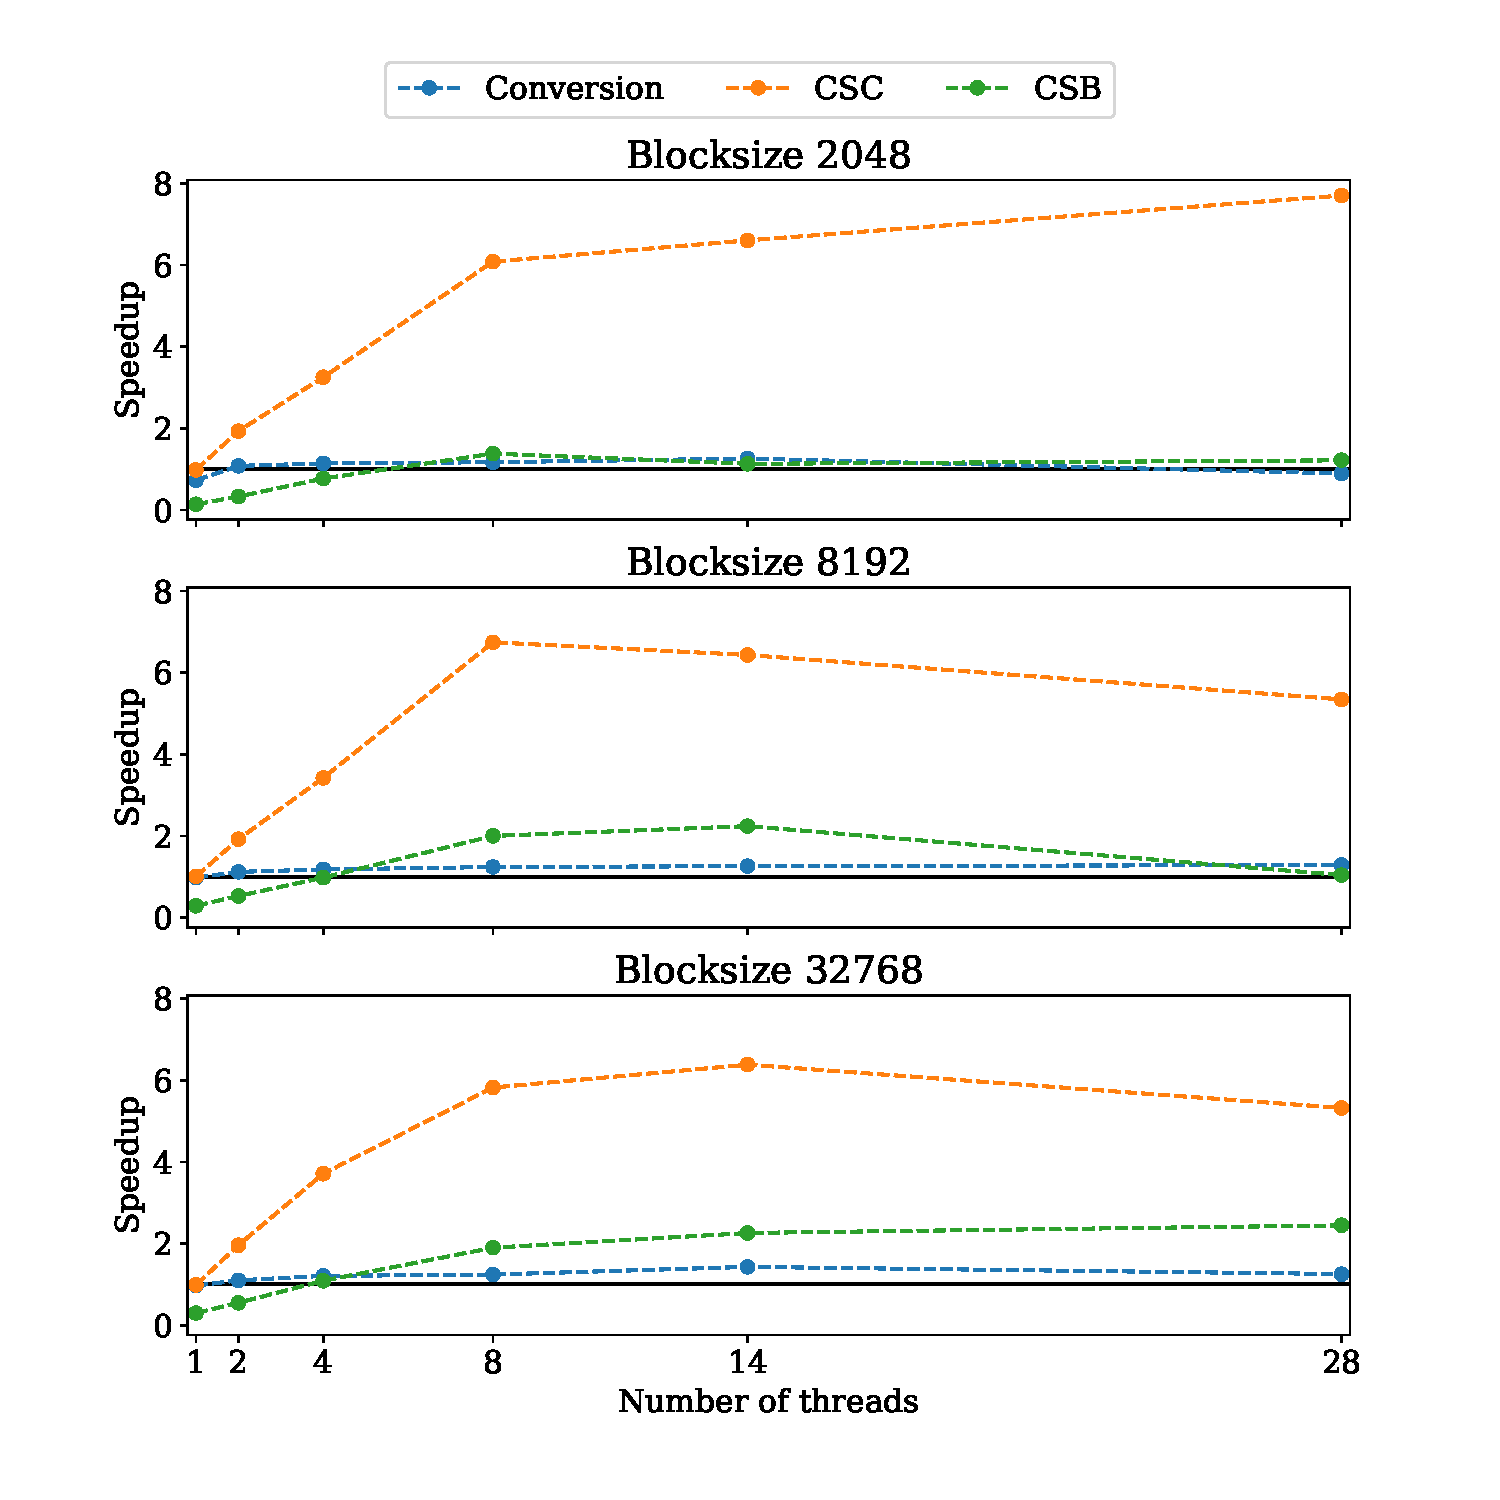
\includegraphics[width=1.4\textwidth]{../plot/sk-2005.pdf}}%
  \caption{Results for the \textit{sk-2005} matrix.}
  \label{fig:sk-2005}
\end{figure}
\begin{figure}
  \centering
  \makebox[\textwidth][c]{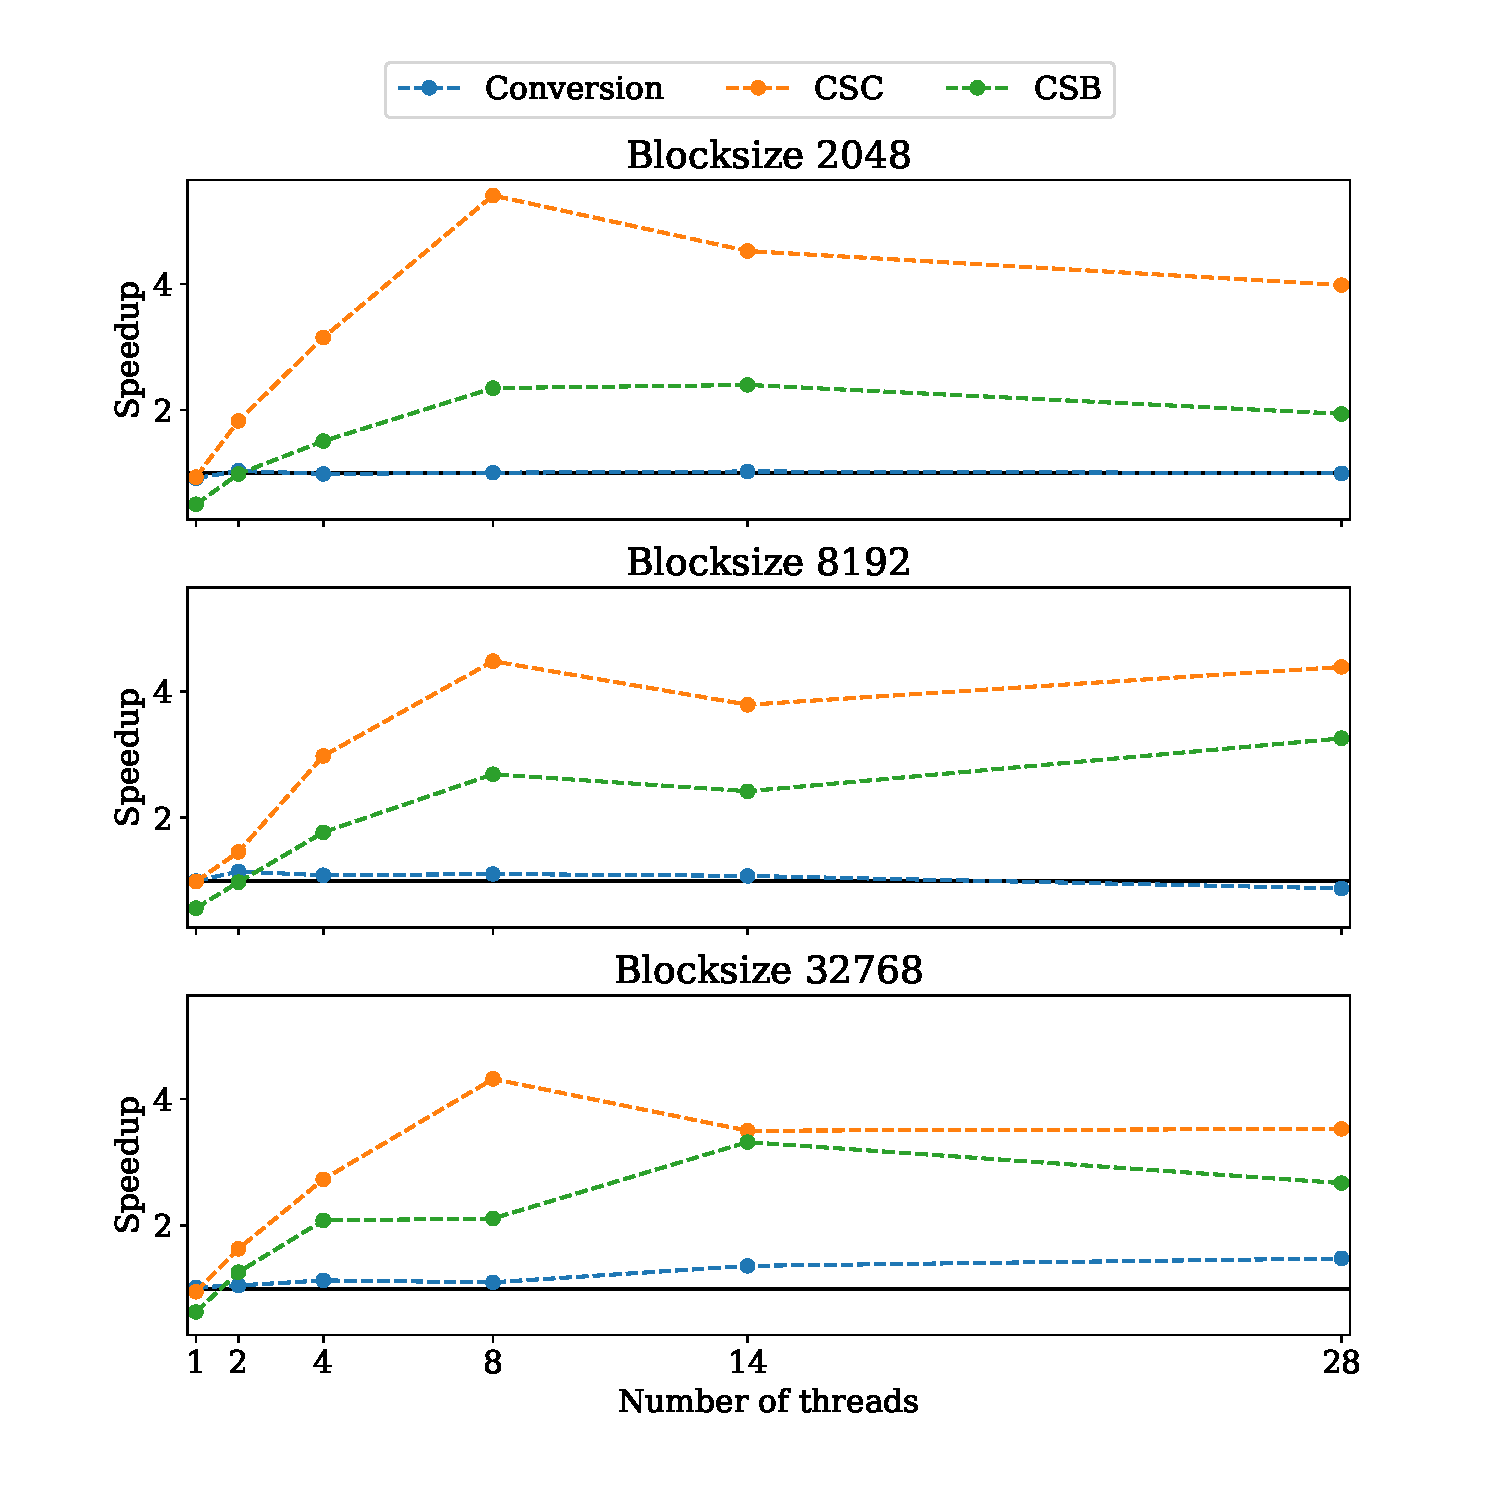
\includegraphics[width=1.4\textwidth]{../plot/twitter7.pdf}}%
  \caption{Results for the \textit{twitter7} matrix.}
  \label{fig:twitter7}
\end{figure}

Over all the results are inconclusive and can't fully be trusted because of
caching effects. If I understand the methods correctly, the CSC multiplication
results should not depend on the blocking factor at all. However, they do
because the CSB sequential routine is executed in between of the CSC sequential
and parallel methods, effecting the caching. 

Nevertheless, there is a general trend we can observe: All methods do not scale
well beyond 14 threads. This can simply be explained by the overhead becoming
to expansive when adding more and more threads. There simply isn't enough work
per thread to justify the amount of overhead generated by each thread when
using a high number of threads.

\end{document}
